% !TeX program = xelatex
% Erzeugt von src/report.py -- nicht direkt bearbeiten, die Zahlen kommen
% aus results/*.json. Aenderungen am Text in src/report.py vornehmen.
\documentclass[11pt,a4paper]{article}
\usepackage[ngerman]{babel}
\usepackage{amsmath,amssymb}
\usepackage{booktabs}
\usepackage{eurosym}
\usepackage[margin=2.5cm]{geometry}
\usepackage{microtype}
\usepackage[htt]{hyphenat}
\usepackage{graphicx}
\usepackage{float}
\usepackage{listings}
\usepackage{xcolor}
\usepackage{caption}
\usepackage[hidelinks]{hyperref}

\graphicspath{{../figures/}}
\captionsetup{font=small,labelfont=bf,skip=6pt}
\setlength{\emergencystretch}{1.5em}

\definecolor{codebg}{gray}{0.96}
\definecolor{codegray}{gray}{0.45}
\lstset{
  basicstyle=\ttfamily\scriptsize,
  backgroundcolor=\color{codebg},
  breaklines=true,
  breakatwhitespace=false,
  columns=fullflexible,
  frame=single,
  rulecolor=\color{codegray},
  framesep=5pt,
  xleftmargin=10pt,
  xrightmargin=4pt,
  language=Python,
  keywordstyle=\color{blue!65!black},
  commentstyle=\color{green!45!black},
  stringstyle=\color{red!55!black},
  showstringspaces=false,
  upquote=true,
}

\title{Kreditrisiko-Analyse\\[0.4em]
\large Vorhersage von Kreditausfaellen und die Wahl der
Entscheidungsschwelle unter ungleichen Kosten}
\author{Chris}
\date{19.~November 2026}

\begin{document}
\maketitle
\thispagestyle{empty}

\begin{abstract}
\noindent
Untersucht wird, wie sich Kreditausfaelle aus acht Merkmalen vorhersagen lassen und wo die Entscheidungsschwelle liegen sollte, wenn ein verpasster Ausfall teurer ist als ein Fehlalarm. Grundlage sind 700 gelabelte Kreditnehmer mit einer Ausfallquote von 26,1~\%. Verglichen werden fuenf Verfahren unter verschachtelter Kreuzvalidierung. Das beste Modell (Logistische Regression + SMOTE) erreicht einen ROC-AUC-Wert von 0,853, bei der Standardschwelle 0,5 aber nur F1 = 0,631. Ursache ist die willkuerliche Schwelle: Mit dem vom Auftraggeber genannten Kostenverhaeltnis von 50:1 (ein verpasster Ausfall kostet 50mal so viel wie eine Pruefung) sinkt die Zahl verpasster Ausfaelle von 40 auf 1 (0,995 statt 0,781 Recall) -- dafuer steigen die Fehlalarme auf 383. Die Treiber sind Beschaeftigungsjahre (schuetzend), Kreditkartenschuld und Schulden-Einkommens-Quote (riskant).
\end{abstract}

\newpage
\tableofcontents
\newpage

\section{Worum es geht}

Aus den Merkmalen eines Kreditnehmers soll vorhergesagt werden, ob er
ausfaellt. Das ist ein Klassifikationsproblem mit \emph{ungleichen Kosten}:
Ein verpasster Ausfall ist teuer, ein Fehlalarm kostet nur eine Pruefung.
Der Bericht misst daher nicht nur die Trennschaerfe, sondern leitet aus einem
Kostenmodell ab, wo die Entscheidungsschwelle liegen sollte.

Drei Fragen stehen im Vordergrund:

\begin{enumerate}
  \item Wie gut lassen sich Kreditnehmer ueberhaupt nach Risiko ordnen?
  \item Welche Merkmale haengen mit einem Ausfall zusammen -- und welche
        nur scheinbar?
  \item Wo sollte die Entscheidungsschwelle liegen, wenn ein verpasster
        Ausfall ein Vielfaches eines Fehlalarms kostet?
\end{enumerate}

\section{Datengrundlage}

Der Datensatz umfasst 1150 Zeilen mit acht Merkmalen (Alter, Bildungsstufe,
Beschaeftigungsjahre, Wohnjahre, Einkommen, Schulden-Einkommens-Quote,
Kreditkartenschuld, sonstige Schulden) und der Zielvariable \texttt{default}.

\textbf{Nur 700 Zeilen tragen ein Label.} Die uebrigen 450 sind ein Block
ohne Zielvariable; sie enthalten ausserdem nur 150 verschiedene
Merkmalsmuster, jedes dreifach wiederholt. Fuer ueberwachtes Lernen sind sie
unbrauchbar und bleiben aussen vor -- sie dienen hoechstens dem Anwenden eines
fertigen Modells.

Von den 700 gelabelten Kreditnehmern sind \textbf{183
ausgefallen (26,1~\%)} -- ein moderat ungleicher
Datensatz, kein Extremfall.

\begin{figure}[H]
  \centering
  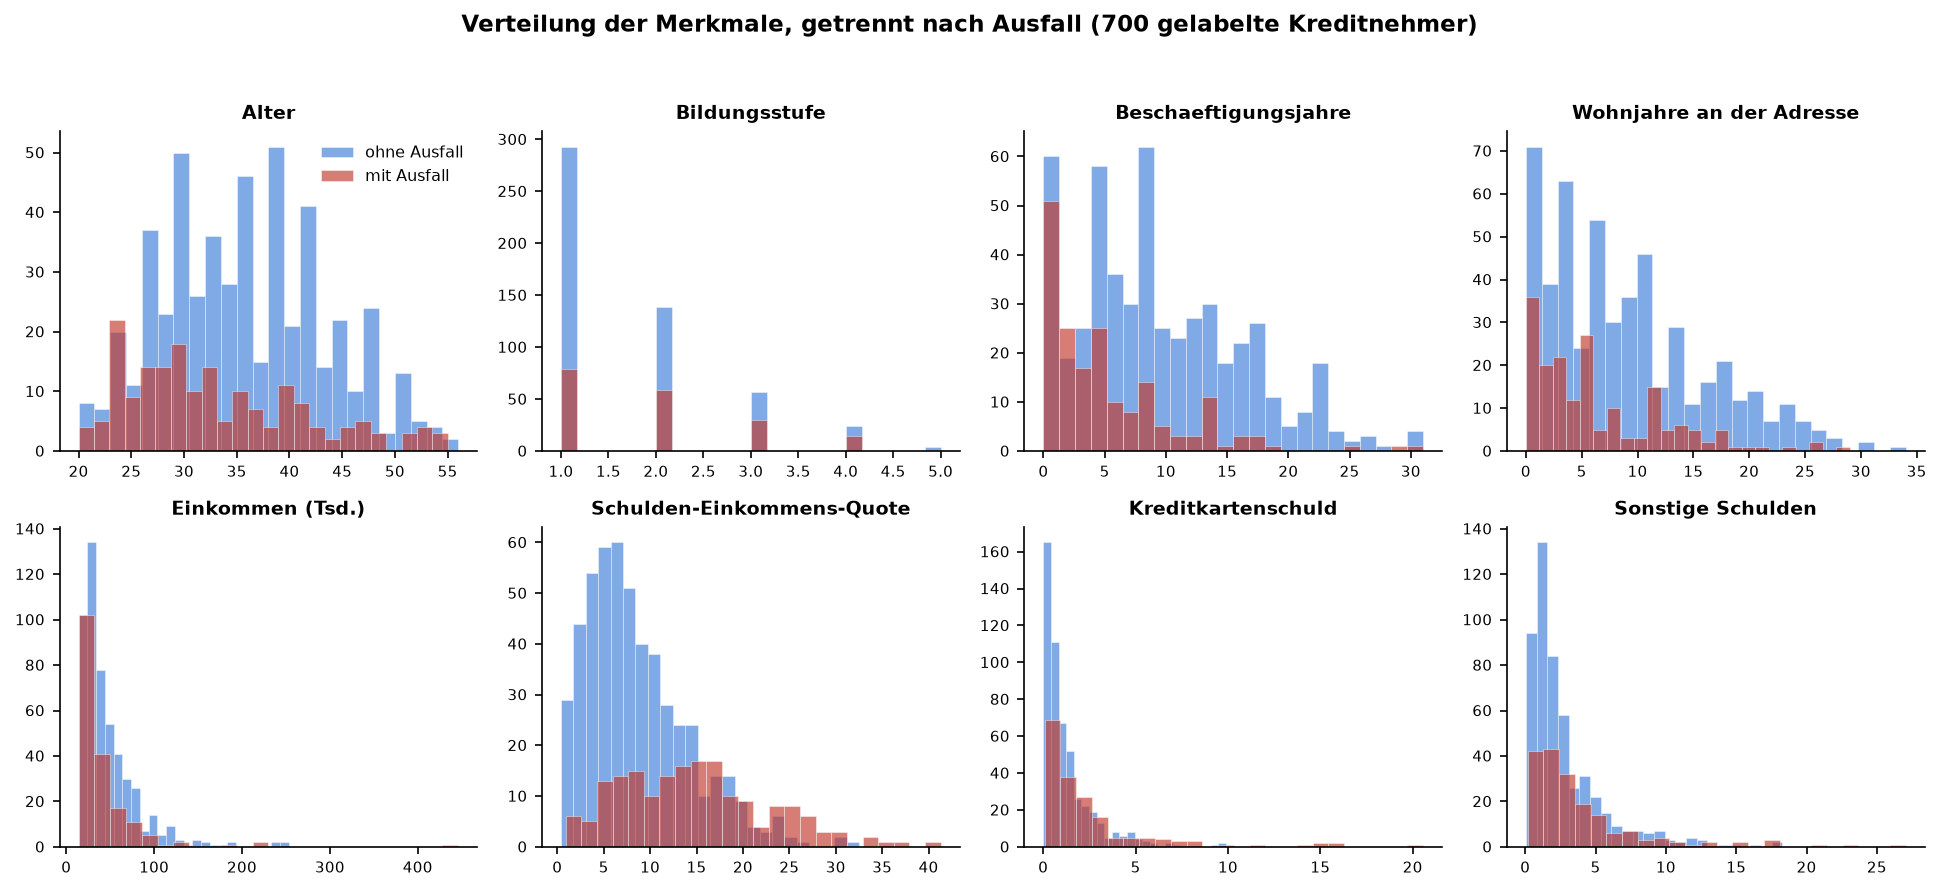
\includegraphics[width=0.90\linewidth]{01_verteilungen.png}
  \caption{Verteilung der Merkmale, getrennt nach Ausfall. Bei der Schulden-Einkommens-Quote und der Kreditkartenschuld liegen die Ausfaller sichtbar rechts, bei den Beschaeftigungs- und Wohnjahren links.}
\end{figure}


\begin{figure}[H]
  \centering
  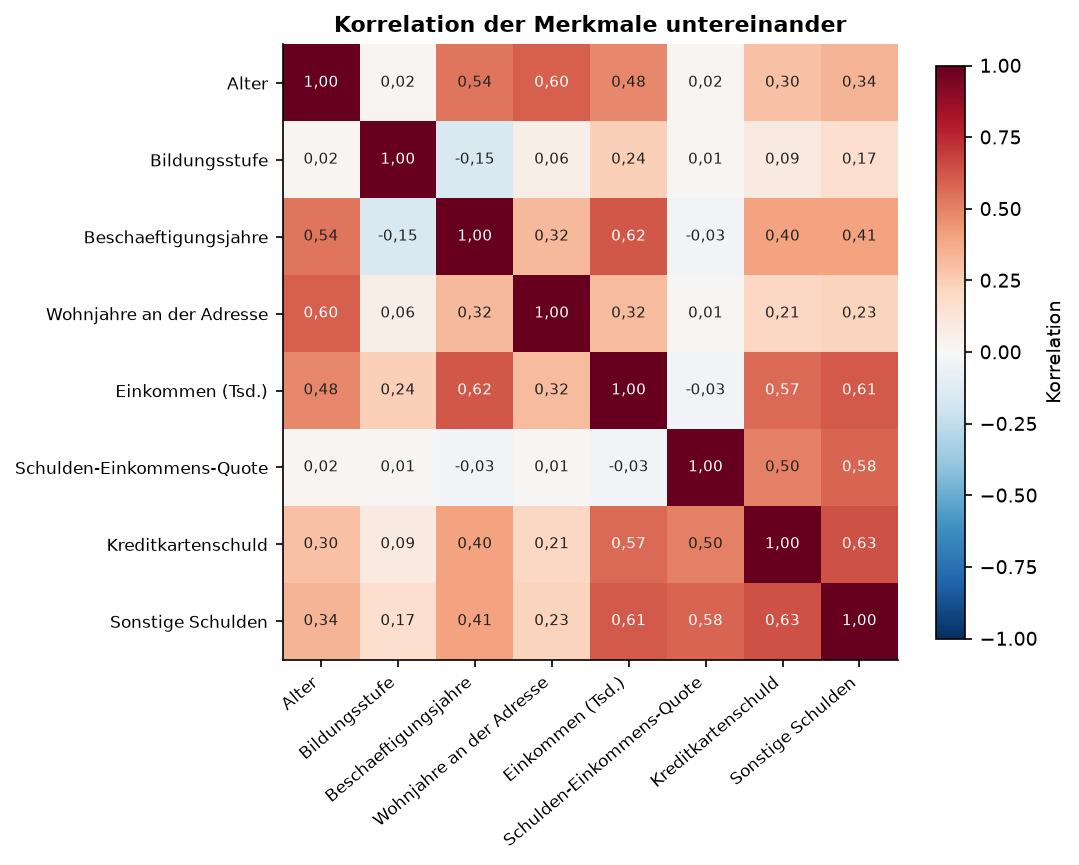
\includegraphics[width=0.90\linewidth]{03_korrelation.png}
  \caption{Korrelation der Merkmale untereinander. Es gibt keine Redundanz, die eine Merkmalsauswahl erzwingen wuerde.}
\end{figure}


\subsection{Was die Merkmale einzeln leisten}

Die Trennschaerfe eines Merkmals allein (AUC; 0,5 bedeutet kein Zusammenhang,
Werte unter 0,5 einen Zusammenhang in die andere Richtung):

\begin{table}[H]
  \centering
  \small
  \begin{tabular}{lr}
    \toprule
    Merkmal & AUC allein \\
    \midrule
    Schulden-Einkommens-Quote & 0,735 \\
    Beschaeftigungsjahre & 0,295 \\
    Kreditkartenschuld & 0,636 \\
    Wohnjahre an der Adresse & 0,389 \\
    Alter & 0,397 \\
    Einkommen (Tsd.) & 0,400 \\
    Sonstige Schulden & 0,587 \\
    Bildungsstufe & 0,574 \\
    \bottomrule
  \end{tabular}
\end{table}


Die \textbf{Schulden-Einkommens-Quote} trennt am besten, gefolgt von der
Kreditkartenschuld. Die Beschaeftigungsjahre wirken in die andere Richtung:
Je laenger jemand beschaeftigt ist, desto geringer das Risiko.

\begin{figure}[H]
  \centering
  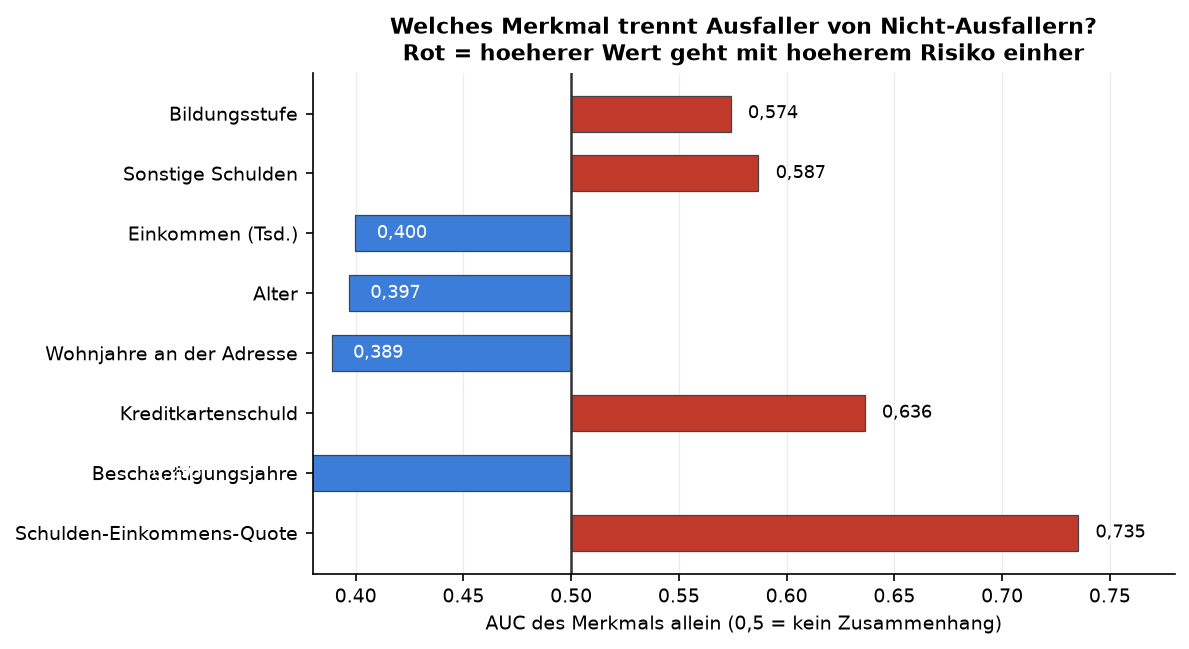
\includegraphics[width=0.90\linewidth]{02_trennschaerfe_einzelmerkmale.png}
  \caption{Trennschaerfe jedes Merkmals allein. Werte ueber 0,5: Ein hoeherer Wert geht mit hoeherem Risiko einher. Werte darunter: mit geringerem.}
\end{figure}


\subsection{Ein scheinbarer Widerspruch, der keiner ist}

Die Ausfallquote steigt mit der Bildungsstufe. Das sieht nach einem starken
Effekt aus, ist aber \textbf{nicht belastbar}:

\begin{table}[H]
  \centering
  \small
  \begin{tabular}{lrrr}
    \toprule
    Bildungsstufe & n & Ausfallquote & KI95 \\
    \midrule
    Stufe 1 & 372 & 21,2 \% & [17,4; 25,7] \\
    Stufe 2 & 198 & 29,8 \% & [23,9; 36,5] \\
    Stufe 3 & 87 & 34,5 \% & [25,3; 44,9] \\
    Stufe 4 & 38 & 36,8 \% & [23,4; 52,7] \\
    Stufe 5 & 5 & 20,0 \% & [3,6; 62,4] \\
    \bottomrule
  \end{tabular}
\end{table}


Die Konfidenzintervalle ueberlappen breit, die oberste Stufe hat nur fuenf
Beobachtungen, und die Korrelation zwischen Bildungsstufe und
Schulden-Einkommens-Quote betraegt 0,009 --
praktisch null. Der Effekt darf nicht als Befund verkauft werden.

\begin{figure}[H]
  \centering
  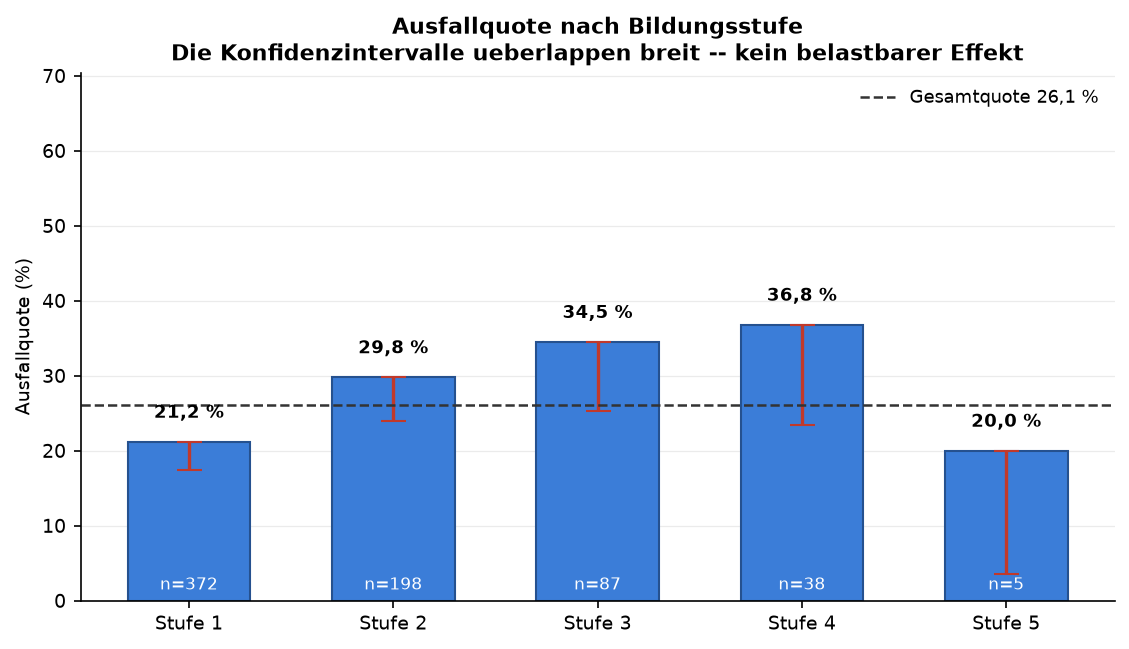
\includegraphics[width=0.90\linewidth]{04_ausfallquote_bildung.png}
  \caption{Ausfallquote je Bildungsstufe mit 95-Prozent-Konfidenzintervall. Der optische Anstieg haelt der Unsicherheit nicht stand.}
\end{figure}


\section{Methodik}

Verglichen werden fuenf Verfahren: Trivialklassifikator (Baseline),
logistische Regression, Random Forest, Gradient Boosting und ein neuronales
Netz -- jeweils ohne und mit Ueberabtastung der Minderheitsklasse (SMOTE).

\paragraph{Verschachtelte Kreuzvalidierung.}
Die Bewertung laeuft ueber 10 aeussere Folds, die Hyperparameterwahl in einem
inneren 3-Fold-Schritt. Damit sieht die Parameterwahl die Bewertungsdaten nie:
Die Kennzahlen sind Messungen, keine Obergrenzen. SMOTE sitzt in der Pipeline
und wirkt nur auf die Trainingsfolds, damit keine kuenstlichen Punkte in die
Bewertung gelangen.

\paragraph{Gepaarter Signifikanztest.}
Die Fold-Ergebnisse je Modell beruhen auf denselben aeusseren Aufteilungen und
sind damit gepaart. Ein Wilcoxon-Vorzeichen-Rang-Test prueft, ob ein
Unterschied groesser ist als die Streuung zwischen den Folds -- strenger als
der optische Vergleich von Fehlerbalken.

\paragraph{Kostenmodell.}
Zwei Fehler sind moeglich: ein verpasster Ausfall (falsch negativ, teuer) und
ein Fehlalarm (falsch positiv, kostet eine Pruefung). Mit einem
Kostenverhaeltnis von $k{:}1$ laesst sich die Schwelle aus dem erwarteten
Nutzen ableiten, statt sie bei 0,5 festzulegen. \textbf{Das vom Auftraggeber
genannte Verhaeltnis betraegt 50:1} -- ein verpasster Ausfall kostet also das
50-fache einer Pruefung. Dieses Leitverhaeltnis steht im Mittelpunkt; die
Verhaeltnisse 1:1, 5:1 und 10:1 bleiben als Vergleichsszenarien daneben
stehen.

\section{Ergebnisse}

\subsection{Modellvergleich}

\begin{table}[H]
  \centering
  \footnotesize
  \begin{tabular}{lrrrrr}
    \toprule
    Modell & F1 & ROC-AUC & PR-AUC & Precision & Recall \\
    \midrule
    Trivial (Mehrheitskl.) (ohne SMOTE) & $0,000 \pm 0,000$ & 0,500 & 0,261 & 0,000 & 0,000 \\
    Trivial (Mehrheitskl.) (mit SMOTE) & $0,000 \pm 0,000$ & 0,500 & 0,261 & 0,000 & 0,000 \\
    Log. Regression (ohne SMOTE) & $0,630 \pm 0,095$ & 0,851 & 0,706 & 0,533 & 0,781 \\
    Log. Regression (mit SMOTE) & $0,631 \pm 0,107$ & 0,853 & 0,706 & 0,536 & 0,775 \\
    Random Forest (ohne SMOTE) & $0,609 \pm 0,081$ & 0,819 & 0,635 & 0,538 & 0,711 \\
    Random Forest (mit SMOTE) & $0,589 \pm 0,083$ & 0,813 & 0,610 & 0,535 & 0,668 \\
    Gradient Boosting (ohne SMOTE) & $0,553 \pm 0,086$ & 0,816 & 0,639 & 0,648 & 0,487 \\
    Gradient Boosting (mit SMOTE) & $0,593 \pm 0,109$ & 0,816 & 0,619 & 0,580 & 0,618 \\
    Neuronales Netz (ohne SMOTE) & $0,496 \pm 0,100$ & 0,807 & 0,619 & 0,569 & 0,448 \\
    Neuronales Netz (mit SMOTE) & $0,581 \pm 0,085$ & 0,792 & 0,595 & 0,518 & 0,667 \\
    \bottomrule
  \end{tabular}
\end{table}


Das beste Ergebnis erzielt \textbf{Logistische Regression + SMOTE} mit F1 = 0,631
($\pm$ 0,107) und ROC-AUC = 0,853.

\begin{figure}[H]
  \centering
  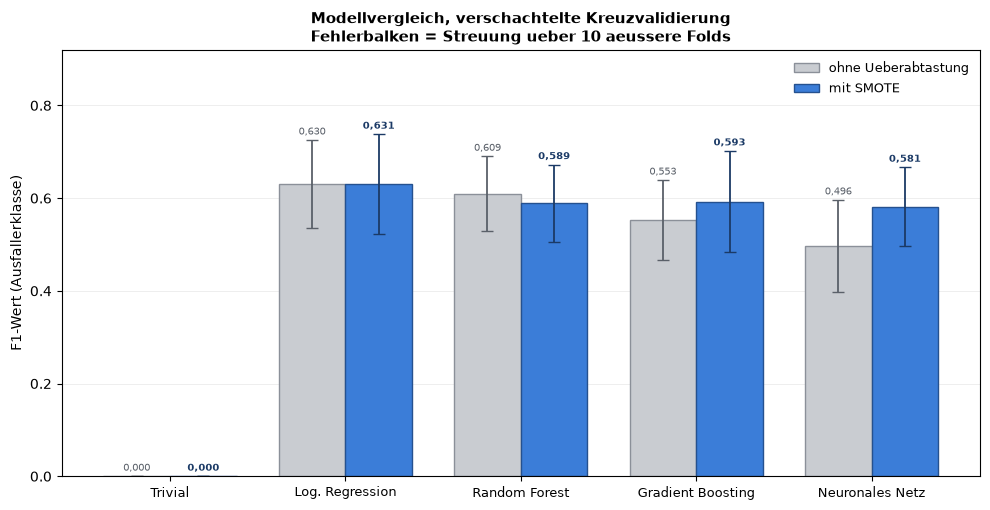
\includegraphics[width=0.90\linewidth]{05_modellvergleich_f1.png}
  \caption{F1-Wert je Verfahren, ohne und mit Ueberabtastung. Fehlerbalken: Streuung ueber die zehn aeusseren Folds.}
\end{figure}


\textbf{Die Modelle ordnen die Kunden deutlich besser, als der F1-Wert
vermuten laesst.} Ein ROC-AUC-Wert von 0,853 bedeutet:
Zieht man einen zufaelligen Ausfaller und einen zufaelligen Nicht-Ausfaller
heraus, wird der Ausfaller in rund 85,3~\% der
Faelle hoeher eingestuft. Der niedrigere F1-Wert entsteht allein durch die
feste Schwelle 0,5 -- dazu Abschnitt~\ref{sec:schwelle}.

\subsection{Bringt Ueberabtastung etwas?}

Fuer die logistische Regression ist der Unterschied nicht unterscheidbar (p = 0,844),
fuer das neuronale Netz signifikant (p = 0,037),
fuer den Random Forest signifikant (p = 0,039).
Ob SMOTE hilft, haengt also von der Konfiguration ab und ist keine allgemeine
Regel.

\subsection{Treiber des Ausfalls}

Standardisierte Koeffizienten der logistischen Regression (untereinander
vergleichbar, weil alle Merkmale dieselbe Skala haben), mit
Bootstrap-Konfidenzintervall und Permutationswichtigkeit (Abfall der ROC-AUC
beim zufaelligen Durchmischen des Merkmals):

\begin{table}[H]
  \centering
  \footnotesize
  \begin{tabular}{lrrrll}
    \toprule
    Merkmal & Koeffizient & Odds-Ratio & KI95 & signifikant & Perm.-AUC \\
    \midrule
    Beschaeftigungsjahre & -1,61 & 0,20 & [-2,07; -1,26] & ja & 0,126 \\
    Kreditkartenschuld & 1,21 & 3,36 & [0,85; 1,69] & ja & 0,039 \\
    Wohnjahre an der Adresse & -0,66 & 0,52 & [-1,04; -0,36] & ja & 0,010 \\
    Schulden-Einkommens-Quote & 0,51 & 1,67 & [0,17; 0,88] & ja & 0,061 \\
    Einkommen (Tsd.) & -0,29 & 0,75 & [-0,85; 0,14] & nein & 0,005 \\
    Alter & 0,27 & 1,31 & [-0,00; 0,53] & nein & 0,007 \\
    Sonstige Schulden & 0,12 & 1,12 & [-0,29; 0,53] & nein & 0,010 \\
    Bildungsstufe & 0,11 & 1,12 & [-0,10; 0,31] & nein & 0,010 \\
    \bottomrule
  \end{tabular}
\end{table}


Die Schulden-Einkommens-Quote und die Kreditkartenschuld erhoehen das Risiko,
Beschaeftigungsjahre und Wohnjahre senken es. Ein Odds-Ratio von
1,67 bei der Schuldenquote heisst: Eine
Erhoehung um eine Standardabweichung vervielfacht die Chance auf einen Ausfall
etwa um diesen Faktor. Einkommen, Alter, sonstige Schulden und Bildungsstufe
sind im Modell \emph{nicht} von Null unterscheidbar.

\begin{figure}[H]
  \centering
  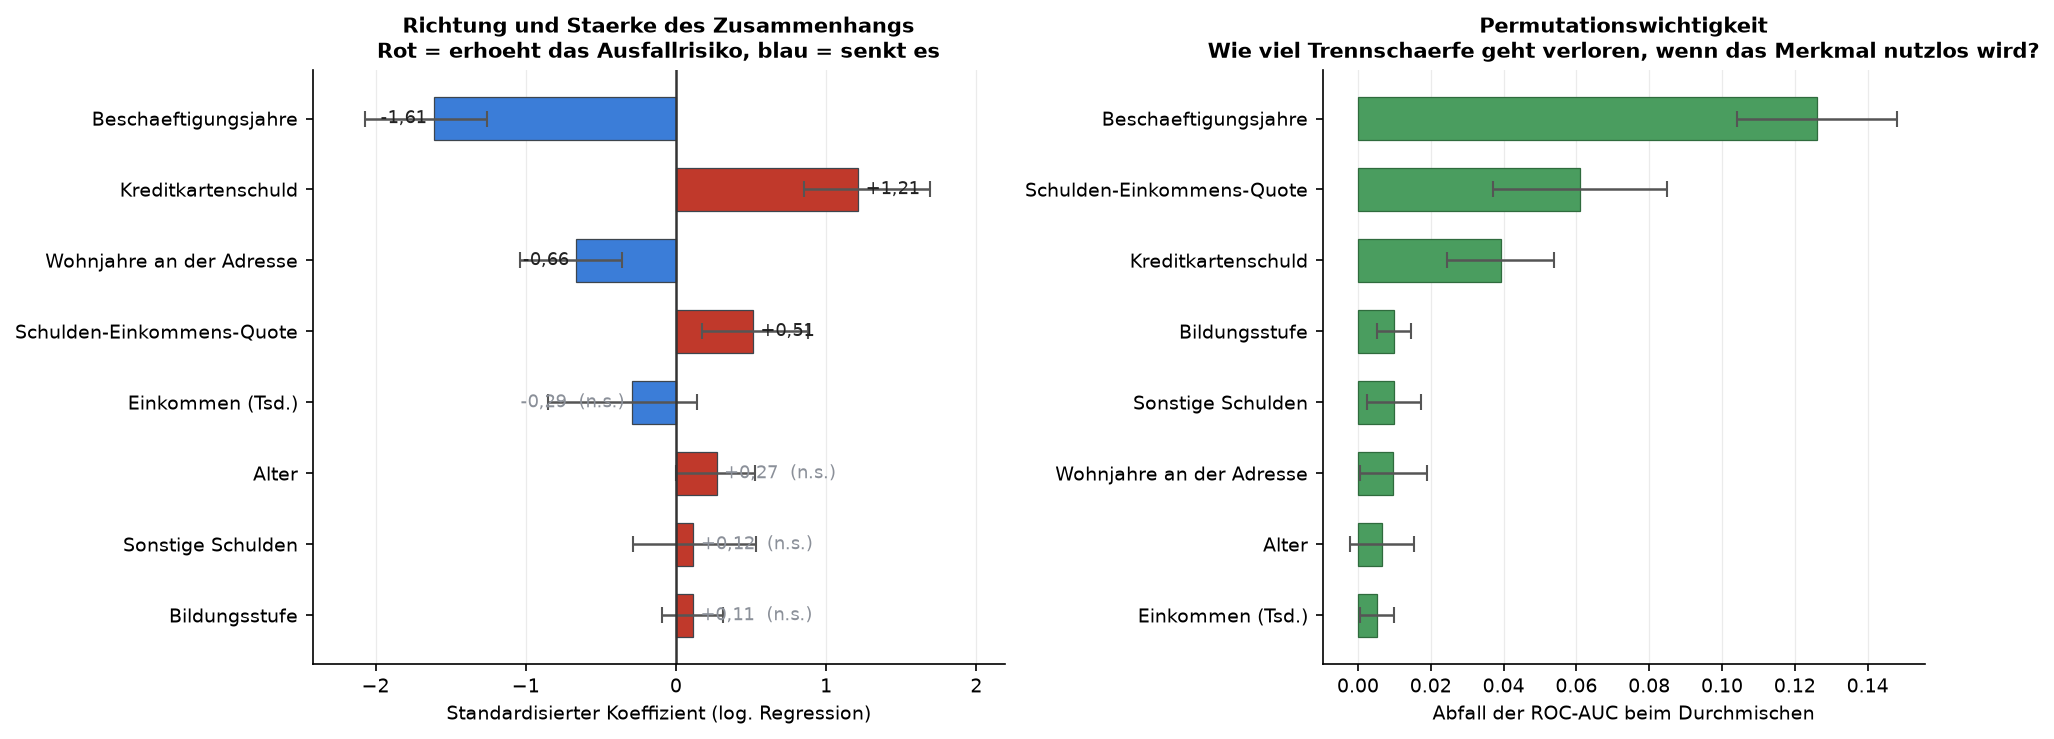
\includegraphics[width=0.90\linewidth]{06_treiber.png}
  \caption{Links: Richtung und Staerke des Zusammenhangs (standardisiert). Rechts: wie viel Trennschaerfe verloren geht, wenn ein Merkmal nutzlos gemacht wird.}
\end{figure}


\section{Schwellenwert und Kosten}
\label{sec:schwelle}

Bei einem Ausfallanteil von 26,1~\% ist die Schwelle
0,5 willkuerlich. Sie wird hier aus dem erwarteten Nutzen abgeleitet:

\begin{table}[H]
  \centering
  \small
  \begin{tabular}{lrrrrrr}
    \toprule
    Schwelle & Precision & Recall & F1 & TP & FP & FN \\
    \midrule
    0,5 (Standard) & 0,526 & 0,781 & 0,629 & 143 & 129 & 40 \\
    1:1 & 0,650 & 0,628 & 0,639 & 115 & 62 & 68 \\
    5:1 & 0,495 & 0,880 & 0,634 & 161 & 164 & 22 \\
    10:1 & 0,394 & 0,945 & 0,556 & 173 & 266 & 10 \\
    50:1 & 0,322 & 0,995 & 0,487 & 182 & 383 & 1 \\
    \bottomrule
  \end{tabular}
\end{table}


\textbf{Der Vergleich zeigt den Gewinn.} Bei der Standardschwelle 0,5 werden
143 Ausfaelle erkannt und \textbf{40 verpasst}. Mit dem vom
Auftraggeber genannten Verhaeltnis \textbf{50:1} -- einem
verpassten Ausfall stehen also 50 Pruefungen gegenueber --
sinkt die optimale Schwelle auf 0,074: Es werden 182
Ausfaelle erkannt, nur noch \textbf{1 verpasst}, bei 383
Fehlalarmen. Der Recall steigt von 0,781 auf 0,995.

Das ist die ehrliche Rechnung: Bei diesem Kostenverhaeltnis ist es
\emph{rational}, eine niedrige Schwelle zu fahren und viele Fehlalarme in
Kauf zu nehmen. Ein Fehlalarm kostet eine Pruefung, ein verpasster Ausfall
50mal so viel -- da lohnt sich der Pruefaufwand fast immer.

Je teurer ein verpasster Ausfall im Verhaeltnis zu einem Fehlalarm, desto
niedriger die optimale Schwelle. Die Szenarien 1:1 bis 10:1 zeigen die
Bandbreite; das Leitverhaeltnis 50:1 ist die belastbare Zahl.

\begin{figure}[H]
  \centering
  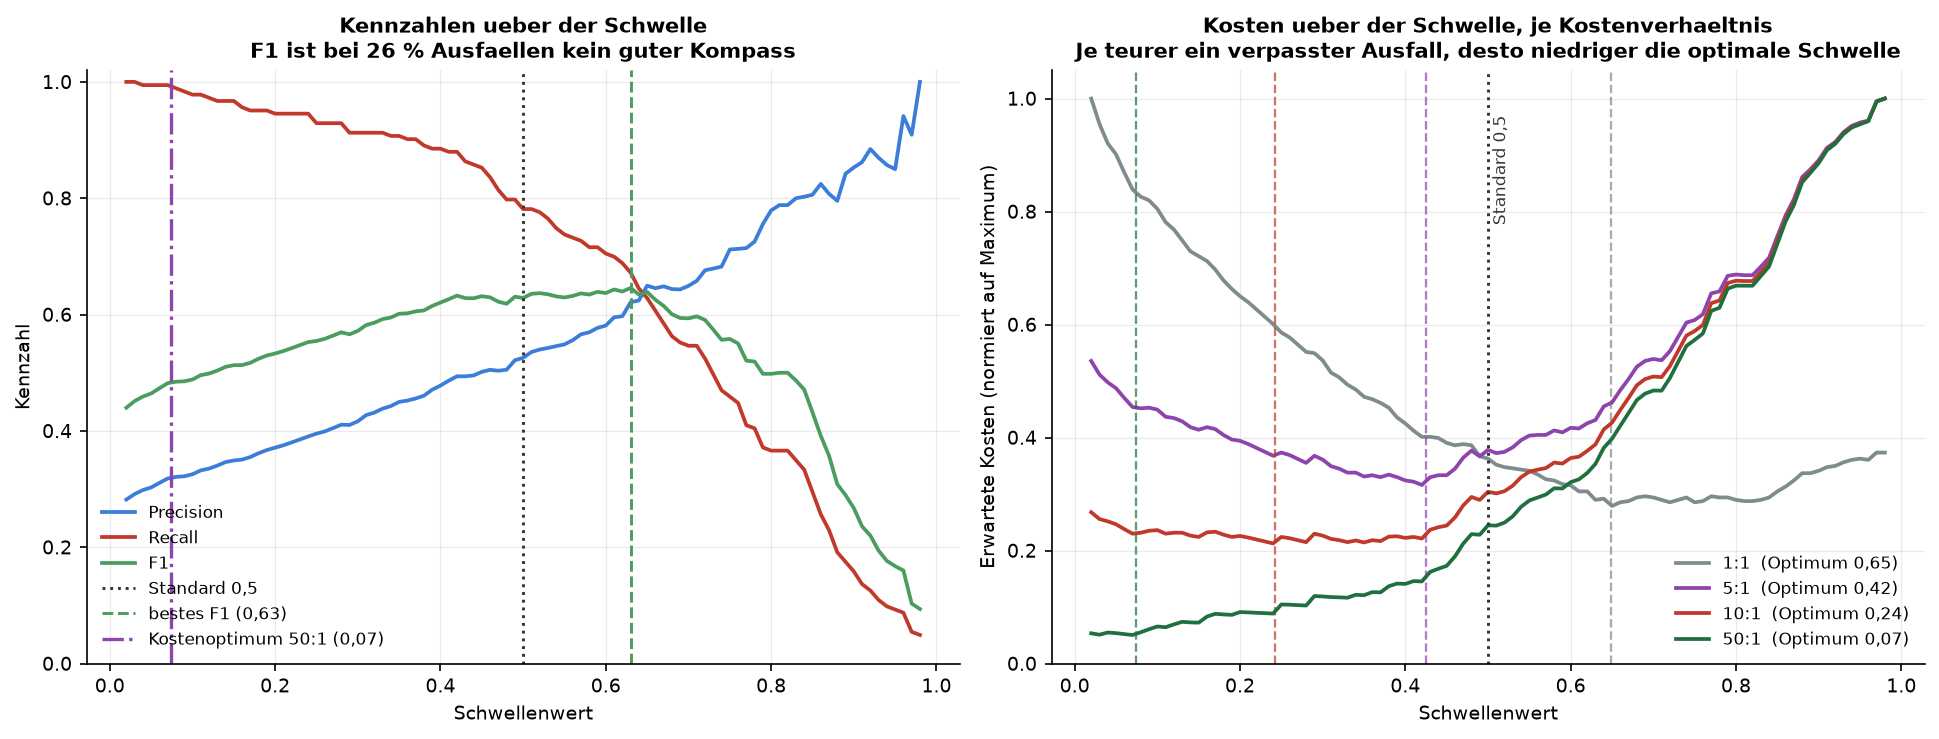
\includegraphics[width=0.90\linewidth]{07_schwellenwerte.png}
  \caption{Links: Precision, Recall und F1 ueber der Schwelle. Rechts: erwartete Kosten je Kostenverhaeltnis -- je teurer ein verpasster Ausfall, desto weiter wandert das Optimum nach links.}
\end{figure}


\begin{figure}[H]
  \centering
  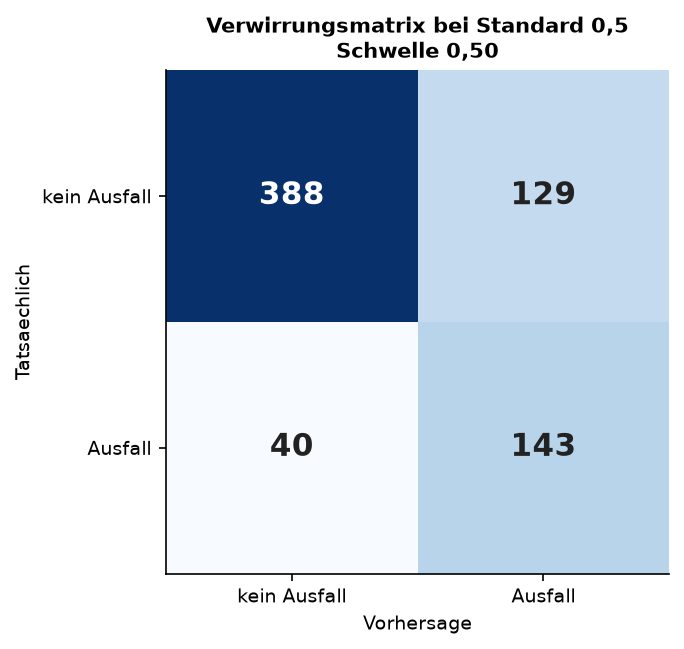
\includegraphics[width=0.55\linewidth]{08_konfusion_050.png}
  \caption{Verwirrungsmatrix bei der Standardschwelle 0,5.}
\end{figure}


\begin{figure}[H]
  \centering
  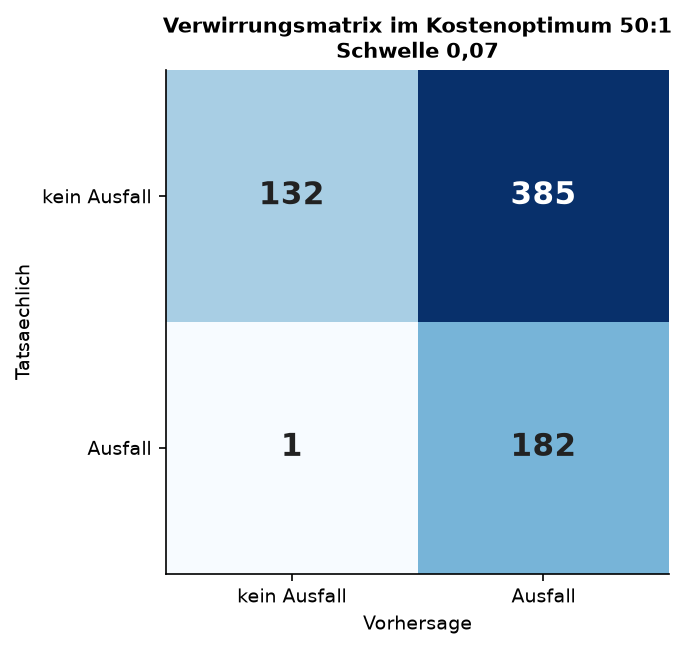
\includegraphics[width=0.55\linewidth]{09_konfusion_kosten.png}
  \caption{Verwirrungsmatrix im Kostenoptimum 50:1. Fast kein Ausfall wird mehr verpasst -- dafuer steigen die Fehlalarme.}
\end{figure}


\section{Grenzen}

\begin{itemize}
  \item \textbf{Nur 700 Zeilen.} Die Kennzahlen tragen Bootstrap-Intervalle
        bzw. Fold-Streuung, sind aber von begrenzter Praezision.
  \item \textbf{Kein Zeitbezug.} Es gibt keinen Beobachtungszeitpunkt, zu
        dem die Merkmale erhoben wurden. Das Modell sagt eine Zugehoerigkeit
        vorher, kein Ereignis zu einem Zeitpunkt.
  \item \textbf{Die 450 ungelabelten Zeilen bleiben ungenutzt.} Sie tragen
        keine Zielvariable; ein halbueberwachter Ansatz waere moeglich, aber
        nur mit zusaetzlicher Annahme.
  \item \textbf{Das Kostenmodell.} Das Verhaeltnis 50:1 ist die vom
        Auftraggeber genannte Relation, keine Messung aus den Daten. Die
        Szenarien 1:1 bis 10:1 zeigen, wie empfindlich das Optimum auf diese
        Annahme reagiert.
  \item \textbf{Keine Ursachenaussage.} Die Koeffizienten zeigen
        Zusammenhang, nicht Wirkung.
\end{itemize}

\section{Reproduktion}

\begin{lstlisting}[language=bash]
python3 data/fetch_data.py       # Rohdaten holen + Form pruefen
python3 src/01_describe.py       # Kennzahlen + Abbildungen
python3 src/02_models.py         # Modellvergleich (verschachtelte CV)
python3 src/03_drivers.py        # Treiberanalyse
python3 src/04_threshold.py      # Schwellenwert + Kostenmodell
python3 src/05_significance.py   # gepaarter Wilcoxon-Test
python3 src/report.py            # dieses PDF (LaTeX ueber Tectonic)
\end{lstlisting}

Die Ergebnisdateien liegen in \texttt{results/} (JSON und CSV im deutschen
Power-BI-Format), die Abbildungen in \texttt{figures/}.


\end{document}
